\documentclass{article}
\usepackage[utf8]{inputenc}
\usepackage{pgfplots}
\pgfplotsset{width=10cm,compat=1.9}
\usepackage{amsmath,amssymb,amsthm}
\usepackage{gensymb}
\usepackage{graphicx}
\usepackage{float}
\usepackage{xcolor}
\usepackage{blindtext}
\usepackage{hyperref}
\usepackage{enumerate}
\usepackage[margin=1in]{geometry}
\hypersetup{
    colorlinks=true,
    linkcolor=blue,
    filecolor=magenta,      
    urlcolor=cyan,
    pdftitle={Overleaf Example},
    pdfpagemode=FullScreen,
    }
\usepackage[slovene]{babel}

\newcounter{example}[section]
\newenvironment{example}[1][]{\refstepcounter{example}\par\medskip
   \noindent \textbf{Naloga~\theexample. #1} \rmfamily}{\medskip}

\newtheorem*{zgled}{Zgled}

\title{Kombinatorika}
\author{Bor Bregant}
\date{\vspace{-5ex}}

\begin{document}

\maketitle
\begin{zgled}
    Na koliko načinov lahko za ravno mizo sedi sedem povabljencev?
\end{zgled}

\textbf{Osnovni izrek kombinatorike ali pravilo produkta}: Če neki proces lahko razdelimo na $k$ zaporednih faz in je prva od faz izvedljiva na $n_1$ načinov, druga na $n_2$ načinov, tretja na $n_3$ načinov, … in $k$-ta na $n_k$ načinov (kjer so izbori med sabo neodvisni), je celotni proces izvedljiv na $n=n_1\cdot \ldots n_k$ načinov.

\begin{zgled}
    Na koliko načinov se lahko oblečemo, če imamo na razpolago dva para čevljev, pet srajc, troje hlač in štiri kravate?\\
    Na koliko načinov lahko damo nase pokrivalo, če imamo na voljo 3 klobuke in dve čepici (\textit{nezdružljivost}).
\end{zgled}


\textbf{Pravilo vsote}: Če izbiramo med $n_1$ možnostmi iz prve množice izborov ali $n_2$ možnostmi iz druge množice naborov in tako naprej (kjer so izbori med sabo neodvisni in nezdružljivi) do $k$-tega nabora, potem je vseh izborov $M=n_1 + \ldots n_k$.

\begin{zgled}
    Do ŠKG lahko pridemo z avtobusi številk 3 ali 5, kjer v obeh primerih naprej prestopimo na 1, 8 ali 25, lahko pa gremo s kolesom ali z avtom. Na koliko različnih način lahko pridemo do šole?
\end{zgled}

\begin{zgled}
    Koliko je vseh različnih metov, če petkrat zapored vržemo kovanec. Predstavi s \textbf{kombinatoričnim drevesom}.
\end{zgled}

\begin{zgled}
    Imamo 25 črk, 5 samoglasnikov. Koliko načinov, če različne črke, če ponavljajo ali pa če morajo biti na prvem mestu soglasniki.
\end{zgled}

\begin{zgled}
    Na razpolago lahko dobimo $5$ modelov mercedesa v $3$ barvah in $4$ modele BMW v $2$ barvah. Med koliko možnostmi izbiramo?
\end{zgled}

\begin{example}
    DN 232a, 248, 254
\end{example}

\begin{zgled}
    Na koliko načinov lahko na polico damo $5$ leposlovnih, $3$ slovarje in $9$ strokovnih knjig, če ni omejitev ali pa če isti tipi morajo iti skupaj.
\end{zgled}








\begin{example}
    DN 232a, 248, 254
\end{example}




\section{Permutacije}

Razporeditve $n$ različnih elementov na $n$ mest, kjer je vrstni red pomemben imenujemo permutacije $n$ elementov. Teh možnosti je $P_n = n! = n (n-1)(n-2)\cdot \ldots \cdot 2\cdot 1$.

\begin{zgled}
    Izračunaj $4!$ in $\frac{n!}{(n-1)!}$.
\end{zgled}

\begin{zgled}
    Koliko besed lahko sestavimo iz črk $ABCDE$, če:\\
    Ni omejitev?\\
    Besede se morajo začeti na $D$\\
    Besede se ne začnejo niti na $A$ niti na $E$\\
    Besede se ne končajo na $DA$
\end{zgled}

\begin{zgled}
    Šestčlanska družina gre v kino. Na koliko načinov se lahko usede v vrsto, če sedita starša skupaj in otroci skupaj. Kaj pa če starša sedita na obeh koncih, otroci pa med njima.
\end{zgled}

\begin{zgled}
    Sedem otrok stoji v vrsti. Na koliko načinov jih lahko prestavimo, če trije najbolj živahni ne smejo biti vsi skupaj.
\end{zgled}

\begin{zgled}
    Preštejmo vse permutacije črk besede $ANANAS$.
\end{zgled}

Permutacij $n$ elementov, kjer se en ponavlja $k_1$-krat, drugi $k_2$-krat in tako naprej, je $P_n ^{k_1,\ldots k_r}=\frac{n!}{k_1 ! \cdots k_r !}$

\begin{zgled}
    Koliko besed iz črk $BOMBAZ$ se ne začne s črko $A$.
\end{zgled}

\begin{zgled}
    Koliko številk iz nabora 5, 6, 7, 8, 9 če brez omejitev ali pa število večje od 70000? \textcolor{gray}{$3\cdot4!$}
\end{zgled}

\begin{zgled}
    Koliko načinov, da $4$ dekleta, $5$ fantov v vrsto, če dekleta skupaj, fantje brez omejitev? \textcolor{gray}{$4!\cdot 5!\cdot 6$ ali pa zlepek dodaten fant torej $4!\cdot 6!$}\\
    Kaj če morajo stati izmenično?
\end{zgled}

\begin{example}
    DN 262, 263, 273, 267, 281, 292.
\end{example}

\begin{zgled}
    Koliko načinov lahko vržemo $3$ cifre in $5$ mož. \textcolor{gray}{$\frac{9!}{3!\cdot 6!}$}
\end{zgled}

\begin{zgled}
    Koliko načinov $5$ ljudi za ravno ali okroglo mizo?
\end{zgled}

\begin{zgled}
    Koliko načinov $2$ avtomobila, $8$ ljudi, $6$ jih ima izpit. \textcolor{gray}{$6\cdot 5\cdot 6!$}
\end{zgled}

\begin{zgled}
    $10$ igrač $3$ otroci. $A$ jih dobi $4$, $B$ jih dobi $3$, $C$ pa $3$. Na koliko načinov si jih lahko razdelijo. \textcolor{gray}{če 10 otrok jih fiksiramo in $10!$ načinov. Naš primer spet fiksiramo igrače, $A$ jih dobi $4$ kot zlepek prvih $4$, a je vseeno, če se v $A$ zmešajo. Torej $\frac{10!}{4!3!3!}$.}
\end{zgled}

\begin{zgled}
    Podobna naloga košarka, $5$ jih je v ekipi, $15$ jih pride na trening. Na koliko načinov $3$ ekipe? \textcolor{gray}{$\frac{15!}{5!5!5!}$}
\end{zgled}

\section{Variacije}

$n$ elementov razporejamo na $r$ mest ($r<n$).

\begin{zgled}
    Na koliko načinov lahko razporedimo 10 dijakov za mizo za 4 osebe.
\end{zgled}

Variacije brez ponavljanja:
\[V_n ^r = N(n-1)(n-2)\cdots (n-r+1)=\frac{n!}{(n-r)!}\]

\begin{zgled}
    Koliko trimestnih števil lahko sestavimo s števkami $1,2,5,8$, če se števke ne smejo ponavljati. Kaj pa če dodamo $0$.
\end{zgled}

\begin{zgled}
    Ponavljanje
\end{zgled}

Variacije s ponavljanjem

\section{Kombinacije}

Na voljo $n$ elementov, izberemo $r$ elementov, vrstni red ni pomemben.

\[\frac{n!}{(n-r)!r!}=\binom{n}{r}=C_n ^r\]

\begin{zgled}
    Koliko načinov 3 kepice izmed 16 vrst , če v kornetu ali skledici? \textcolor{gray}{kornet vrstni red pomemben $16\cdot 15\cdot 14$ skleda vrstni red ni pomemben $\frac{16!}{(16-3)!3!}$.}
\end{zgled}

\begin{zgled}
    Na koliko načinov lahko izberemo $3$ dijake iz razreda $22$ deklet in $5$ fantov. Kaj pa $2$ dekleti in enega fanta. 
\end{zgled}

\begin{zgled}
    Naloga z igračami lažje $\binom{10}{4}\cdot\binom{6}{3}\cdot\binom{3}{3}$.
\end{zgled}

\begin{zgled}
    $12$ deklet, $18$ fantov. Na koliko načinov lahko določimo otvoritveni par.
\end{zgled}

Hitro računanje binoma: $\binom{98}{4}=\frac{98\cdot 87\cdot 96\cdot 95}{4\cdot 3\cdot 2 \cdot 1}$. (enako cifer zgoraj kot spodaj)

\subsection{Lastnosti binomskih simbolov}

\begin{enumerate}[i]
    \item $\binom{n}{0}=1$ Med $n$ elementi jih izberemo $0$

            Dokaz $\binom{n}{0}=\frac{n!}{(n-0)!\cdot 0!} =1$
    \item $\binom{n}{1}=n$
    \item   Simetričnost $\binom{n}{r}=\binom{n}{n-r}$
    
            Dokaz $\binom{n}{r}=\frac{n!}{(n-r)!r!}=\frac{n!}{(n-(n-r))!\cdot (n-r)!}=\binom{n}{n-r}$

            Posledica $\binom{n}{n}=\binom{n}{n-n}=\binom{n}{0}=1$
    \item   Aditivnost $\binom{n}{r}+\binom{n}{r+1}=\binom{n+1}{r+1}$
    
            Dokaz s Pascalovim trikotnikom
  \end{enumerate}

\begin{zgled}
    Izračunaj $\binom{n}{n-2}$ in $\binom{200}{197}+\binom{200}{198}$\textcolor{gray}{$= \binom{201}{198}= \binom{201}{3}=\frac{201\cdot 200 \cdot 199}{3\cdot 2\cdot 1}$}.
\end{zgled}

\begin{zgled}
    Poenostavi $\binom{n+1}{n}$ in $\binom{n+1}{k+1}:\binom{n}{k}$
\end{zgled}

\begin{zgled}
    Reši enačbo $C_{n+2}^3 =n\cdot C_{n+1}^1$.
\end{zgled}

\begin{example}
    DN Računanje binoma 346č, 347ač, 348ac, 349
\end{example}

%\begin{zgled}
%    350
%\end{zgled}

%\begin{example}
%    DN 351, 356
%\end{example}

\subsection{Binomski izek}

Vpeljava z $(a+b)^i$ in Pascalovim trikotnikom.

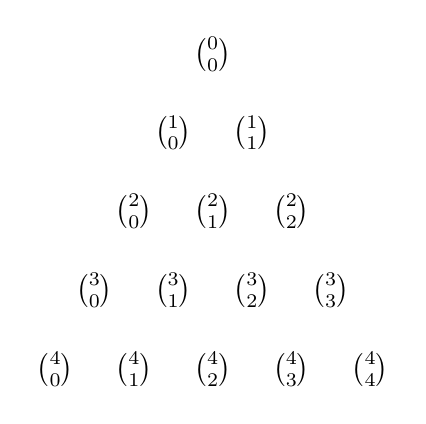
\begin{tikzpicture}
    \foreach \n in {0,...,4} {
      \foreach \k in {0,...,\n} {
        \node at (\k-\n/2,-\n) {${\n \choose \k}$};
      }
    }
\end{tikzpicture}

\[\left(a+b\right)^n = \binom{n}{0}a^n +\binom{n}{1}a^{n-1}b + \binom{n}{2}a^{n-2}b^2+\ldots + \binom{n}{n}b^n\]

\begin{zgled}
    Izračunaj $(x^2-\sqrt{2})^6$.
\end{zgled}

\begin{zgled}
    Izračunaj 17. člen v razvoju $(2a-b^2)^23$. \textcolor{gray}{Predznak +, $\binom{23}{16}(2a)^7(b^2)^16$}
\end{zgled}

DN 380, 381

\end{document}